% Drawing 57/06-1 -- folder 57, batch 06, archive page 104 (PDF page 105).
% Transcription: en marge, un petit tableau incliné, à colonnes, où se lisent $\mathrm{Div}^+$ et quelques mots illisibles
% Kind: tilted table in the margin. Method 2 (schematic redraw from the facsimile). Status: partial.
% Notes: Tilted frame, its corners computed once: the top edge from the top left corner to the top right corner (broken where a word crosses it, as on the page), the right edge down to the bottom right corner, the bottom edge curving back to the bottom left corner, the left edge (which starts only below the first row on the page; the short stroke above it is drawn apart); the inner bottom line ending at the bottom right corner. Four column lines, the first ending on the bottom edge. The heavy stroke across the two right columns is drawn. Div^+ placed where "Div" is visible in the lower right cell, along his writing. Still differs: the other words in the cells (x+, f, +x and the like) are not legible enough to be composed and are left out; the two right column lines are approximate (faint and partly overwritten). Redrawn 2026-11-09 (issue 128): to check again.
% Coordinates: 1 unit = 1 mm = 1/100 of the crop width (bbox in page fractions: [0.1, 0.67, 0.31, 0.83]).
% Redrawn by Claude (claude-opus-5-5), issue #73, 2026-11-09; not checked by a human; not compiled (no TeX in the session).
% Rights: reproduces part of the work -- behind RENDER_TRANSCRIPTS, never published by itself.
\documentclass[tikz,border=3pt]{standalone}
\usepackage{amsmath,amssymb}
\usetikzlibrary{patterns,arrows.meta}
\tikzset{pencil/.style={black!45}, struck/.style={black!35}, mark/.style={circle,draw,inner sep=1.3pt}, pt/.style={circle,fill,inner sep=0.9pt}, opt/.style={circle,draw,fill=white,inner sep=1.1pt}}
\begin{document}
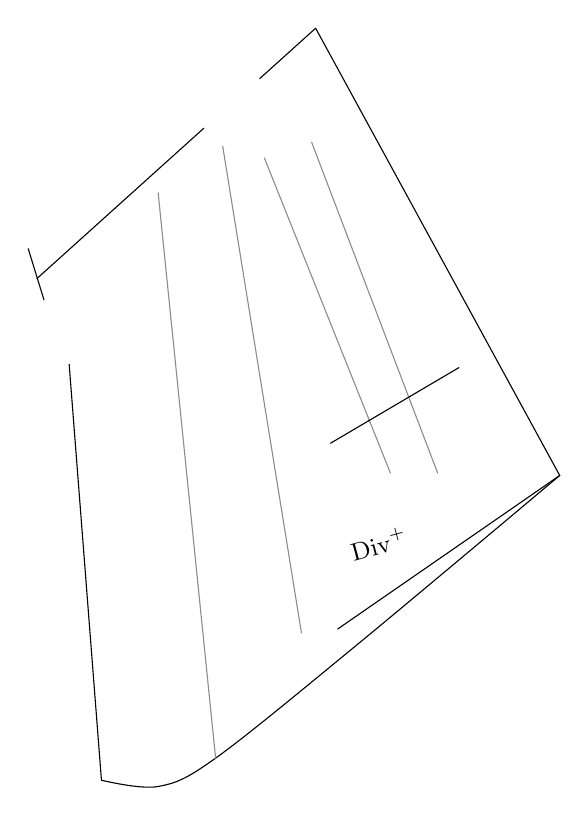
\begin{tikzpicture}[x=1mm,y=1mm,line cap=round,line join=round,font=\scriptsize]
\draw (9.1,-37.3) -- (30.3,-18.2);
\draw (37.4,-11.9) -- (44.5,-5.5);
\draw (44.5,-5.5) -- (75.5,-62.3);
\draw plot[smooth, tension=0.55] coordinates {(75.5,-62.3) (50,-83.6) (31.8,-98.2) (24.5,-101.8) (17.3,-101)};
\draw (13.2,-48.2) -- (17.3,-101);
\draw (8,-33.5) -- (10,-40);
\draw (47.3,-81.8) -- (75.5,-62.3);
\draw[pencil] (24.5,-26.4) -- (31.8,-98.2);
\draw[pencil] (32.7,-20.5) -- (42.7,-82.3);
\draw[pencil] (38,-22) -- (54,-62);
\draw[pencil] (44,-20) -- (60,-62);
\draw (46.4,-58.2) -- (62.7,-48.6);
\node[inner sep=1pt,rotate=15] at (52.5,-71) {\small $\mathrm{Div}^+$};
\end{tikzpicture}
\end{document}
